
%
%%----------------------------------------------------------------


\section{Modelo de información: Módulo Estructura Educativa}
\subsection{Módulo Estructura Educativa: Descripción general}

En la figura~\ref{fig:estructuraEducativa} se muestra la estructura de información que manejará el módulo Estructura Educativa.

\begin{figure}[htbp!]
	\begin{center}
		\fbox{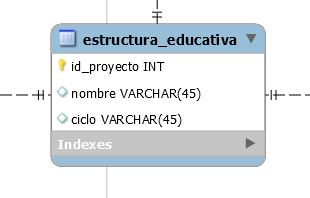
\includegraphics[width=.5\textwidth]{images/clases/EstructuraEducativa.PNG}}
		\caption{Modelo de información del módulo Estructura educativa.}
		\label{fig:estructuraEducativa}
	\end{center}
\end{figure}

%--------------------------------------------------------------------------------
\begin{BusinessEntity}{estructuraEducativa}{Estructura educativa}
	
	\Battr{nombre}{Nombre}{\tdFrase}{Es el nombre con el que se registra el edificio}{\requerido}{\longitudMax{50}{caracteres}}{Caracteres admitidos: [A-Z] $|$ [a-z] $|$ [1-9] $|$ \_ $|$ $-$ $|$ [á,é,é,ó,ú]  $|$ [Á,É,Í,Ó,Ú] $|$ \textvisiblespace.}
	
	\Battr{cicloEscolar}{CicloEscolar}{\tdCatalogo}{Es el nombre del ciclo escolar, el cual está formado por el ciclo escolar / 1 o 2 según corresponda.}{\requerido}
	
\end{BusinessEntity}


%--------------------------------------------------------------------------------

\subsection{Módulo Grupos: Descripción general}
En la figura~\ref{fig:grupos} se muestra la estructura de información que manejará el módulo Grupos.

\begin{figure}[htbp!]
	\begin{center}
		\fbox{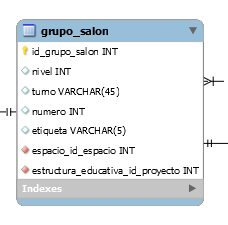
\includegraphics[width=.5\textwidth]{images/clases/GrupoEspacio.png}}
		\caption{Modelo de información del módulo Grupos.}
		\label{fig:grupos}
	\end{center}
\end{figure}

%--------------------------------------------------------------------------------
\begin{BusinessEntity}{grupo}{Grupo}
	
	\Battr{turno}{Turno}{\tdPalabra}{Es el turno al cual pertencerá el grupo. De estos sólo existen CM y CV}{\requerido}{\longitudMax{2}{caracteres}}{Caracteres admitidos: CM $|$ CV.}
		
	\Battr{numero}{Número}{\tdPalabra}{Es el número consecutivo que se le da a los grupos, después de indicar el nivel y turno. Este será el número que lo diferencia de otro grupo }{\requerido}{\longitudMax{2}{caracteres}}{Caracteres admitidos: [1-99] .}

	\Battr{nombre}{Nombre}{\tdFrase}{Es el nombre con el que se registra el grupo. Este es la concatenación del nivel + turno + numero}{\requerido}{\longitudMax{5}{caracteres}}{Caracteres admitidos: CM $|$ CV $|$ [a-z] $|$ [1-9].}
	
		
\end{BusinessEntity}


%--------------------------------------------------------------------------------

\subsection{Módulo Asociación de profesores: Descripción general}
En la figura~\ref{fig:asociacionProfesores} se muestra la estructura de información que manejará el módulo Asociación de Profesores.

\begin{figure}[htbp!]
	\begin{center}
		\fbox{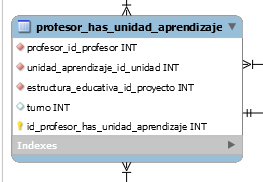
\includegraphics[width=.5\textwidth]{images/clases/ProfesorUnidadAprendizaje.png}}
		\caption{Modelo de información del módulo Asociación de profesores.}
		\label{fig:asociacionProfesores}
	\end{center}
\end{figure}

%--------------------------------------------------------------------------------
\begin{BusinessEntity}{grupo}{Grupo}
	
	\Battr{turno}{Turno}{\tdPalabra}{Es el turno al cual pertencerá el grupo. De estos sólo existen CM y CV}{\requerido}{\longitudMax{2}{caracteres}}{Caracteres admitidos: CM $|$ CV.}
	
	\Battr{numero}{Número}{\tdPalabra}{Es el número consecutivo que se le da a los grupos, después de indicar el nivel y turno. Este será el número que lo diferencia de otro grupo }{\requerido}{\longitudMax{2}{caracteres}}{Caracteres admitidos: [1-99] .}
	
	\Battr{nombre}{Nombre}{\tdFrase}{Es el nombre con el que se registra el grupo. Este es la concatenación del nivel + turno + numero}{\requerido}{\longitudMax{5}{caracteres}}{Caracteres admitidos: CM $|$ CV $|$ [a-z] $|$ [1-9].}
	
	
\end{BusinessEntity}

%--------------------------------------------------------------------------------